\section{Demonstrationsversuch}
	
	\subsection{Methoden}
				
			\begin{figure}[ht]
				\centering
				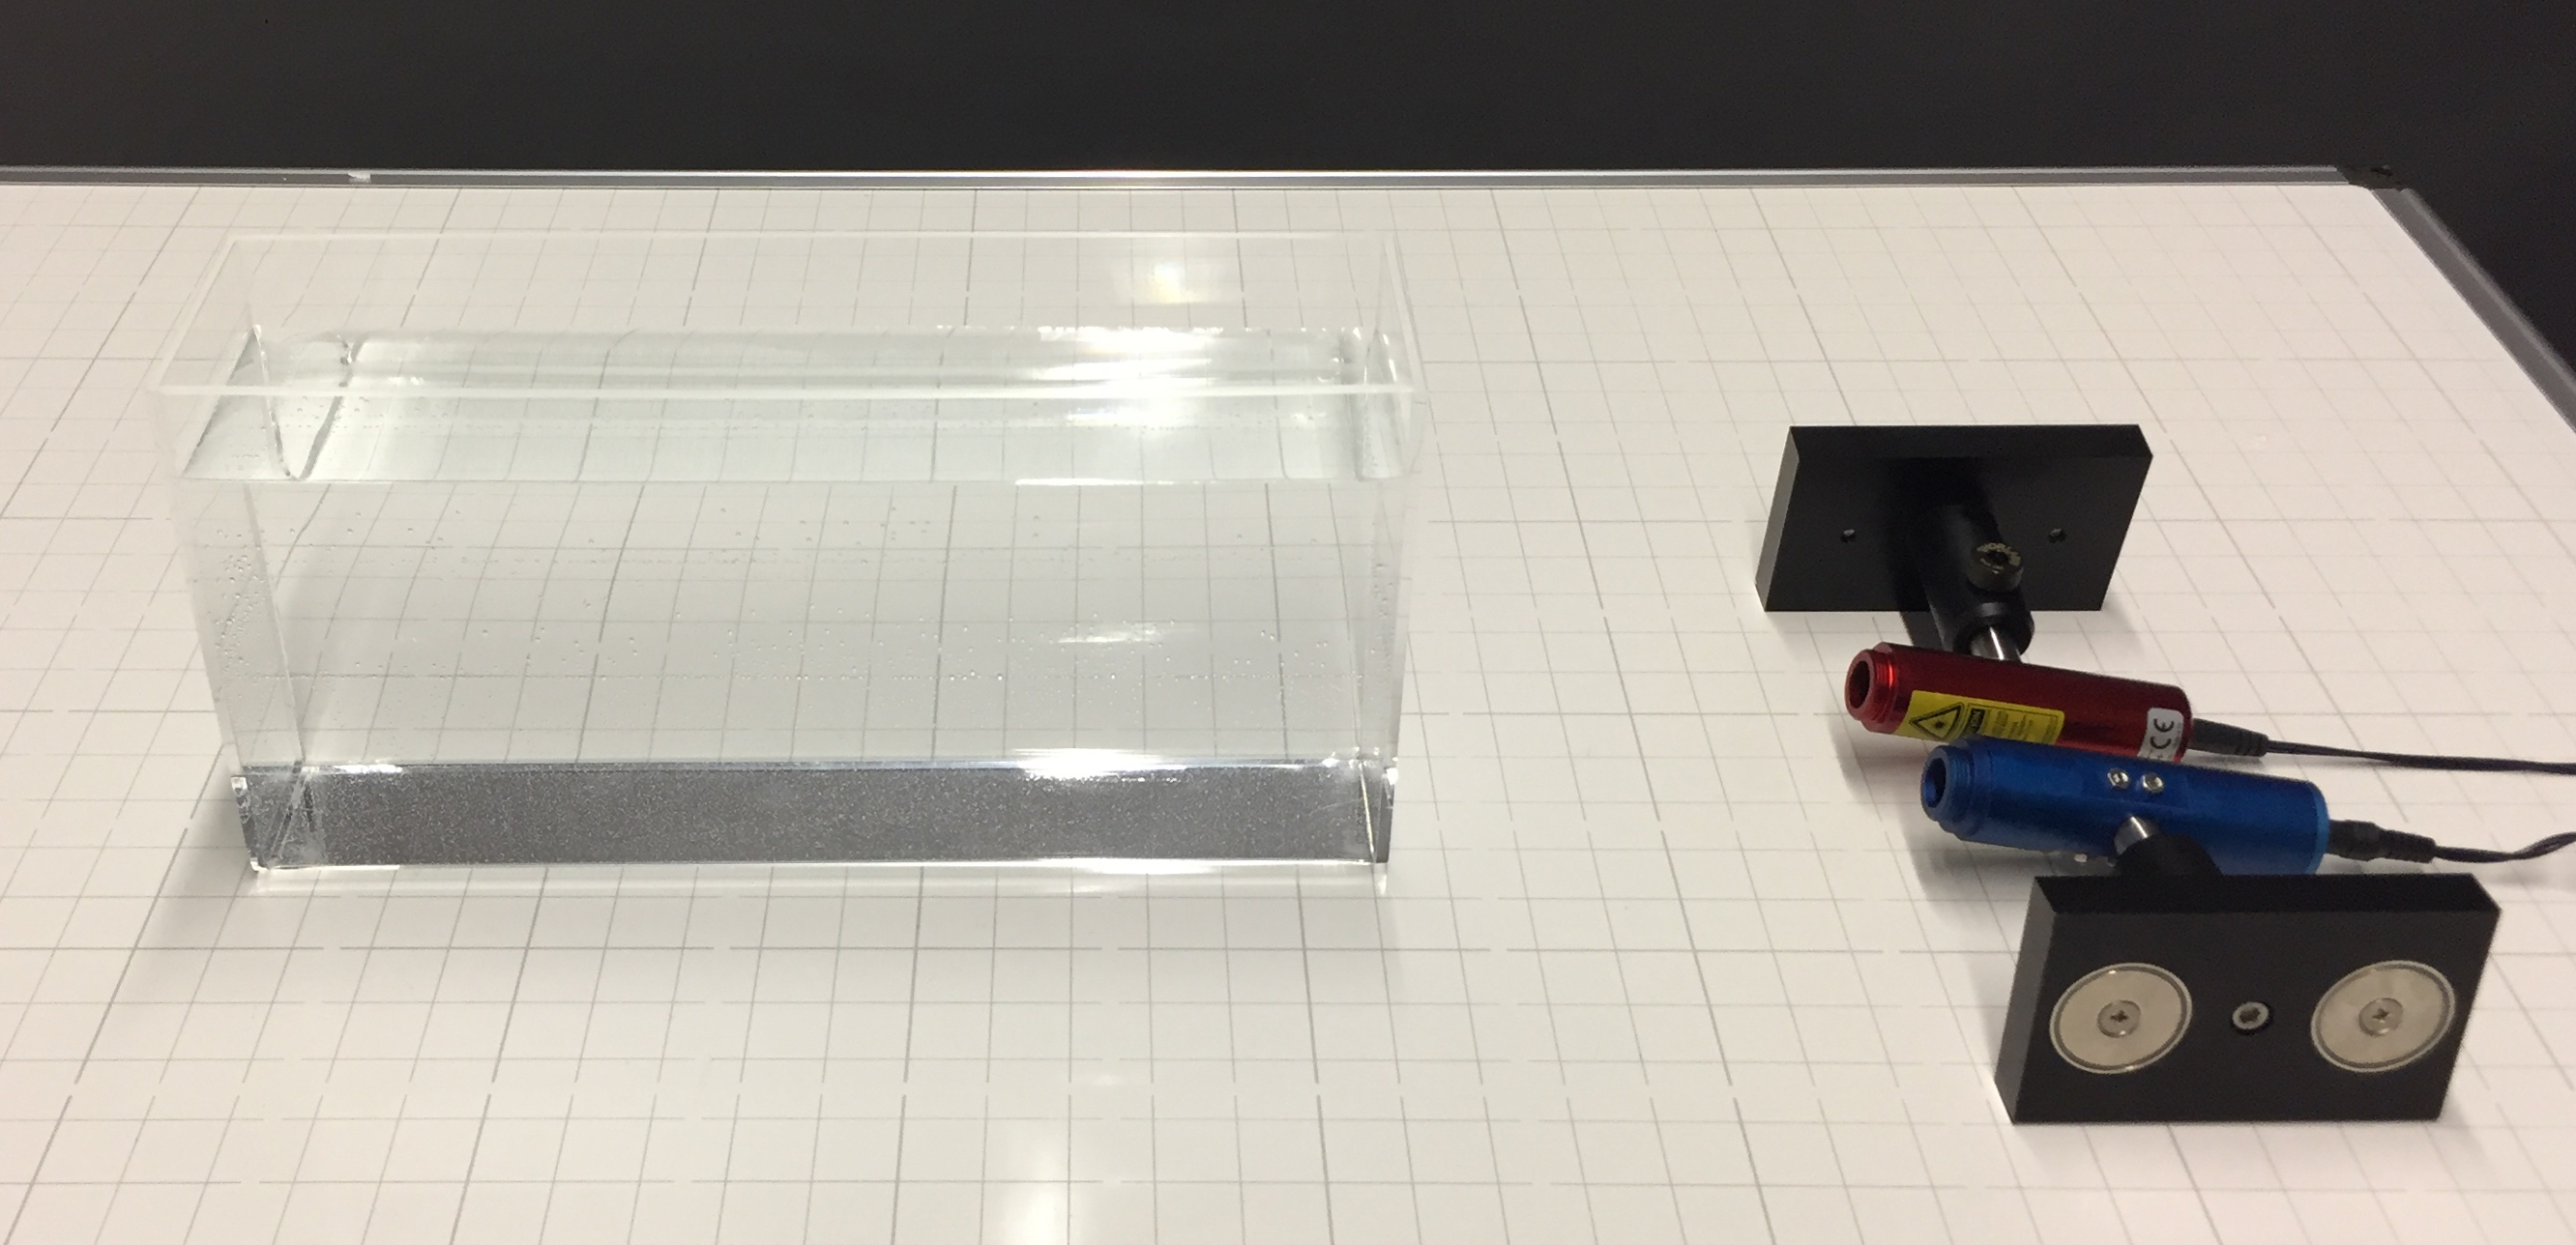
\includegraphics[width=\textwidth]{bilder/aufbau1.jpg}
				\caption{Aufbau des Demonstrationsversuches.\cite{WWU}}
				\label{fig:Aufbau1}	
			\end{figure}
			Der Versuchsaufbau ist in Abbildung \ref{fig:Aufbau1} graphisch dargestellt.
			Zu erkennen sind ein mit Salzwasser gefülltes Glasgefäß und darauf gerichtete Laser. 
			Das Wasser wurde so bearbeitet, dass der Salzgehalt von oben nach unten größer wird.
			
			Im Wesentlichen werden für diesen Versuch nur beide bzw. nur einer der Laser in Betrieb genommen und der Strahlengang, welcher zunächst schräg nach oben in das Gefäß eintreten soll, beobachtet.
			Abhängig von der Krümmung des Strahlengangs in der Salzlösung lässt sich eine Aussage über den dortigen Brechungsindex $n_\text{Salz}$ machen.
			
	\subsection{Durchführung}
		
		Nach Inbetriebnahme beider Laser, wobei einer durch die Salzlösung strahlt und der andere entlang der Glaswand, ließ sich das in Abbildung \ref{fig:Beobachtung1} dargestellte Bild erkennen.
		\begin{figure}[ht]
			\centering
			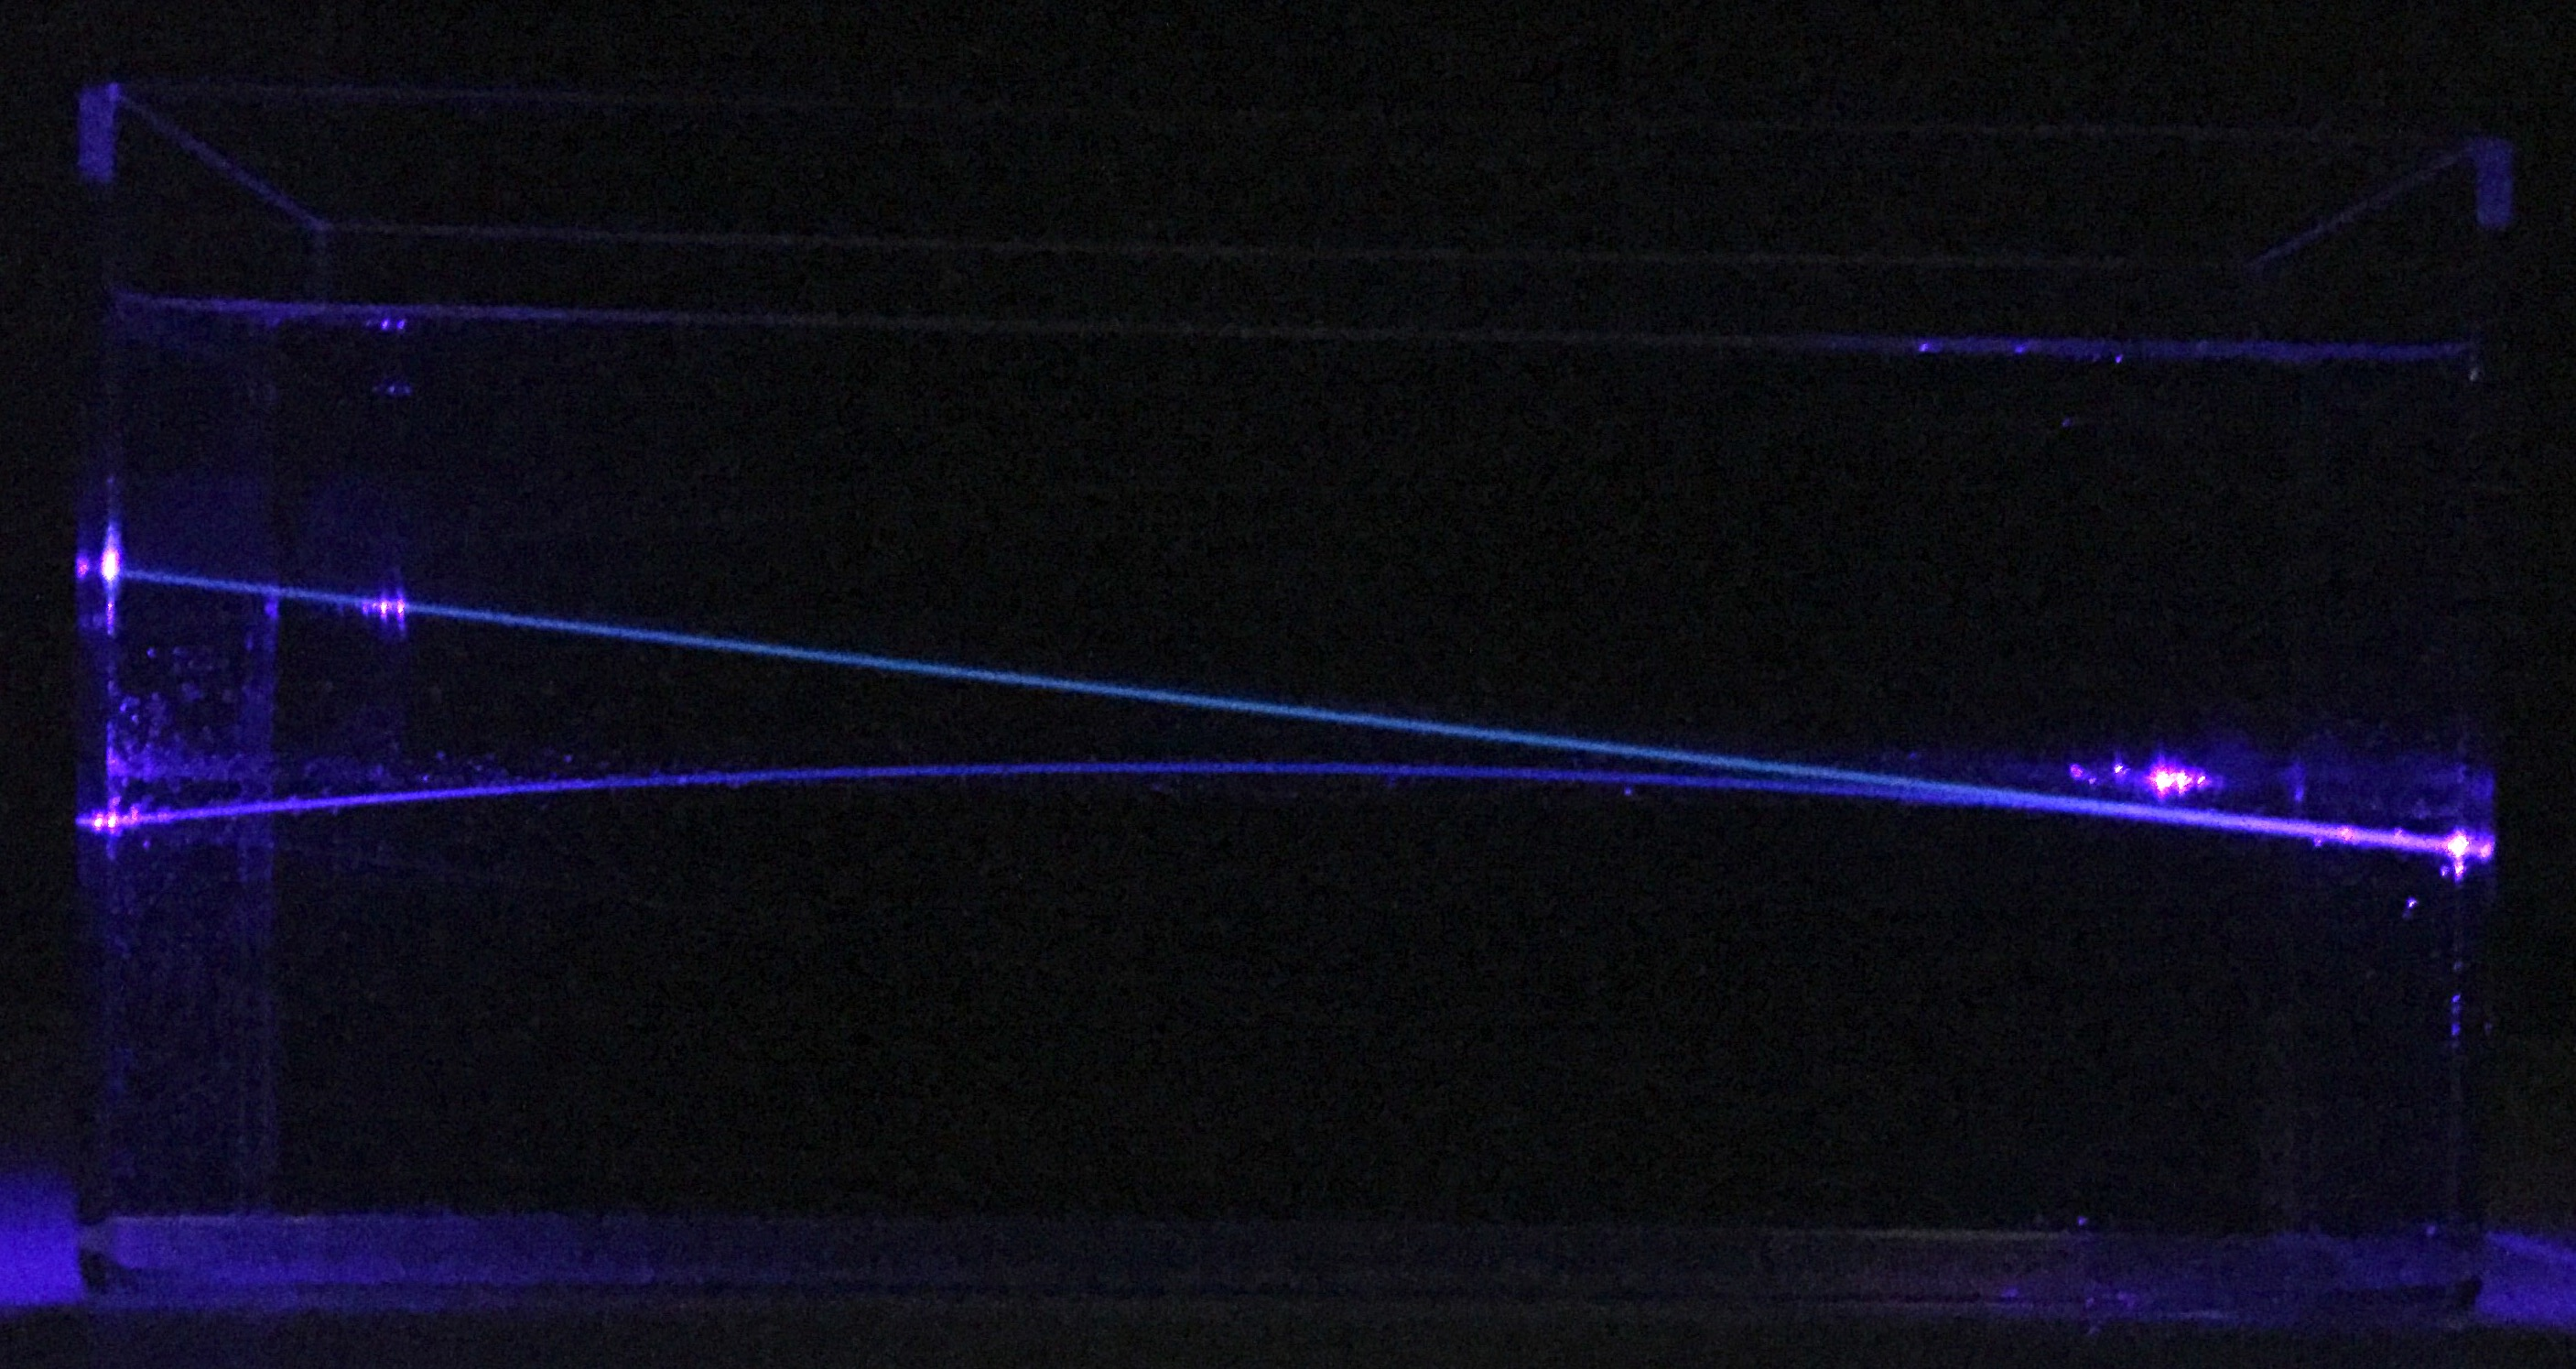
\includegraphics[width=\textwidth]{bilder/beobachtung1.jpg}
			\caption{Strahlengang durch das Salzwasser (gebrochen) und entlang der Wand des Glasgefäßes (gerade).\cite{WWU}}
			\label{fig:Beobachtung1}	
		\end{figure}
		Hierbei war eine nach unten gerichtete Krümmung des Laserlichts in der Salzlösung erkennen. 
		
	\subsection{Diskussion}
		
		Die bei dem Versuch beobachtete Krümmung führt zu der Annahme, dass der Brechungsindex  $n_\text{Salz}$ der Salzlösung nicht konstant ist.
		Um zu bestimmen, ob dieser mit der Tiefe des Lichts in der Salzlösung größer oder kleiner wird dient das Snelliussche Brechungsgesetz: $n_1\sin{\alpha_1} = n_2\sin{\alpha_2}$.
		Diese Winkel entsprechen denen, die zwischen dem Strahlengang und der Normalen durch den Eintrittspunkt an der Grenzfläche zwischen Glasgefäß und Luft liegen.
		Daraus folgt, dass wenn der Strahl, wie beobachtet, zu der Normalen hin gekrümmt wird, gerade $n_\text{Salz} > n_\text{Luft}$ gilt.
		Und da dieser Strahlengang sich mit steigender Tiefe weiter krümmt, folgt dass durch den steigendem Salzgehalt auch der Brechungsindex $n_\text{Salz}$ größer wird.
		Somit lassen sich die Beobachtungen über die Theorie erklären.
